\documentclass[11pt,openany]{book}
% #1-Asignatura
% #2-Curso
% #3-Nombre
% #4-Link
% #5-Foto

\newcommand{\portada}[5]{
    \begin{titlepage}
        \begin{center}
            \vspace*{0.5cm}
            
            % Titulo con #1 lo mas grande posible
            {\Huge \textbf{#1}}

            
            \vspace{0.5cm}
            \LARGE
            Curso #2 
            
            \vspace{1cm}
            
            \Huge{\textbf{Grupo Viterbi}}

            \vspace{1cm}
            
\includegraphics[width=0.6\textwidth]{assets/Img/UGR-Logo.png}
            
            \vspace{0.5cm}

            \huge
            PRÁCTICA 5- PROGRAMACIÓN DINÁMICA
            
            \Large
            \vspace{1cm}
            \textbf{Integrantes:}  \\ 
             % Array con los nombres de los integrantes y el correo
             \begin{center}
                \begin{tabular}{c c }
                    \textbf{Miguel Ángel De la Vega Rodríguez} & miguevrod@correo.ugr.es \\
                    \textbf{Alberto De la Vera Sánchez} & joaquinrojo724@correo.ugr.es \\
                    \textbf{Joaquín Avilés De la Fuente} & adelaveras01@correo.ugr.es \\
                    \textbf{Manuel Gomez Rubio} & e.manuelgmez@go.ugr.es \\
                    \textbf{Pablo Linari Perez} & e.pablolinari@go.ugr.es
                \end{tabular}
             \end{center}
            \vspace{0.8cm}
            
            
            \large
             \vspace{1cm}
            Facultad de Ciencias UGR\\
            Escuela Técnica Ingeniería Informática UGR\\
            Granada\\
            #2 
            
        \end{center}
    \end{titlepage}
}



\usepackage{assets/formulas}
\usepackage{float}
\hbadness=10000 % Suppress Underfull \hbox warnings

%========================================|Indice|===============================================%

\begin{document}
\portada{Algorítmica}{2023-2024}{Miguel Ángel De la Vega Rodríguez}{https://github.com/Miguevrgo/}{github.png}
\tableofcontents % Índice
\newpage %Salto de pagina tras el Indice


%======================================|Documento|==============================================%
\chapter{Autores}
\begin{itemize}
      \item \textbf{Miguel Ángel De la Vega Rodríguez:} 20\%
            \begin{itemize}
                  \item Algoritmos del Viajante
                  \item Redacción memoria sección Viajante
            \end{itemize}
      \item \textbf{Joaquín Avilés De la Fuente:} 20\%
            \begin{itemize}
                  \item Programacion SumaMax (DyV)
                  \item Estudio eficiencia teórica algoritmos específicos y DyV
                  \item Tests de eficiencia
            \end{itemize}
      \item \textbf{Alberto De la Vera Sánchez: } 20\%
            \begin{itemize}
                  \item Redacción \LaTeX
                  \item Estudio de umbrales teóricos y empíricos de DyV
                  \item Graficas y ajustes
            \end{itemize}
      \item \textbf{Manuel Gomez Rubio} 20\%
            \begin{itemize}
                  \item Programacion SumaMax (Kadane)
                  \item Programacion Losetas
            \end{itemize}
      \item \textbf{Pablo Linari Pérez:} 20\%
            \begin{itemize}
                  \item Programacion SumaMax (Kadane)
                  \item Programacion Losetas
            \end{itemize}
\end{itemize}

\chapter{Equipo de trabajo}

\begin{itemize}
      \item \textbf{Miguel Ángel De la Vega Rodríguez:} (Ordenador donde se ha realizado el computo)
            \begin{itemize}
                  \item AMD Ryzen 7 2700X 8-Core
                  \item 16 GB RAM DDR4 3200 MHz
                  \item NVIDIA GeForce GTX 1660 Ti
                  \item 1 TB SSD NvMe
                  \item Debian 12 Bookworm
                  \item Compilador GCC 12.2.0
            \end{itemize}
\end{itemize}
% Viajante es el apartado 6, incluir capitulos antes
\chapter{Viajante} % Migue
En esta sección se analiza todo aquello referente al cuarto problema propuesto,
el problema del viajante. Siguiendo las directrices indicadas, se han estudiado
y diseñado diferentes algoritmos "Greedy" que aproximan el problema, con el objetivo
final de comparar cual nos proporciona mejores resultados en cuanto a términos
de eficiencia y precisión. Para determinar esto último, también cabe destacar
detalles de menor importancia como la complejidad de los algoritmos, la estabilidad
frente a distintas entradas o la posibilidad de mejora de los mismos mediante la
elección de distintos puntos de partida o con mejoras posteriores como pueden ser 
aquellas que proporcionan algoritmos como $\lambda$-opt o genéticos.
\\ \\
De aqui en adelante, describiremos por secciones los algoritmos implementados y 
al final proporcionaremos una sección comparativa sobre la cual nos basaremos
para determinar conclusiones, en particular, elegiremos el algoritmo cuya
solución consideremos más conveniente. En lo que sigue se muestra únicamente
el resultado obtenido por el algoritmo sin mejoras posteriores, este tipo de mejoras
suponen una pequeña desvirtuación del objetivo de encontrar el mejor algoritmo y 
es por ello, que su uso se limita a la conclusión final.

\section{Algoritmo \textit{Nearest Neighbour}}
Tal y como el nombre indica, el primer algoritmo implementado no es nada más, ni 
nada menos que el primer algoritmo que probablemente se le puede ocurrir a cualquier
persona que se enfrente a este problema. La idea es sencilla e intuitiva, nos 
dan un conjunto de puntos y queremos encontrar el camino más corto que los recorra,
para ello, \textbf{elegimos} un punto inicial y a partir de ese punto, en un proceso 
iterativo, elegimos en cada paso el siguiente punto más cercano al actual, o lo que 
es lo mismo, el punto para el cual la distancia al punto actual es la menor (No confundir
con el punto para el cual la distancia total es la menor, ya que, aunque parecido, no es 
lo mismo). Este proceso se repite hasta que todos los puntos han sido visitados.
\\ \\
A continuación se proporciona la implementación propuesta del algoritmo en cuestión:
\begin{lstlisting}[language=C++]
vector<Point> nearestNeighborTSP(const vector<Point>& points) {
  vector<Point> path;
  vector<bool> visited(points.size(), false);
  path.reserve(points.size());
  path.emplace_back(points[0]);
  visited[0] = true;

  for (int i = 0; i < points.size() - 1; ++i) {
    double minDistance = numeric_limits<double>::max();
    int nearestNeighbor = -1;
    for (int j = 0; j < points.size(); ++j) {
      if (!visited[j]) {
        double distance = path[i].distanceTo(points[j]);
        if (distance < minDistance) {
          minDistance = distance;
          nearestNeighbor = j;
        }
      }
    }
    path.emplace_back(points[nearestNeighbor]);
    visited[nearestNeighbor] = true;
  }

  return path;
}
\end{lstlisting}
Como se puede apreciar, se ha hecho uso de un vector de puntos visitados (Programación 
dinámica) para evitar visitar un punto más de una vez, esto no supone una complejidad
notable, sin embargo, si que supone una gran mejora en términos de eficiencia.

\section{Algoritmo \textit{Ordenación}}
Como el nombre indica, este algoritmo consiste en ordenar los puntos de partida de
acuerdo a un criterio especifico (en nuestro caso los hemos ordenado por la coordenada
x de menor a mayor, teniendo en cuenta también para puntos cercanos en x, la coordenada y).
Una vez ordenados los puntos, simplemente recorremos el vector de puntos en el orden
en el que se encuentren, de esta forma, el camino total trata de reducir cruces y distancias
con la idea intuitiva de que si dos puntos están cerca en el plano, probablemente, la 
distancia que se recorra al pasar por ellos, sea mínima. Como veremos en el siguiente 
algoritmo y en la conclusión, esto en la práctica no es del todo cierto. Primero veamos 
la implementación del algoritmo:
\begin{lstlisting}[language=C++]
vector<Point> orderedTSP(const vector<Point>& points) {
      vector<Point> tour;
      tour.reserve(points.size());
      copy(points.begin(), points.end(), back_inserter(tour));
      sort(tour.begin(), tour.end());
        
      return tour;
}      
\end{lstlisting}
Como se puede apreciar, la implementación es muy sencilla, simplemente se copian los puntos
de partida a un vector auxiliar, se ordenan y se devuelve el vector ordenado, sin embargo
cuando vemos el resultado de la ejecución, nos damos cuenta de que aunque los puntos
esten muy cerca respecto a la coordenada x, los saltos que se dan en la coordenada y
pueden ser muy grandes, lo que hace que el camino total sea mucho mayor de lo esperado,
además para cerrar el camino, la distancia es la máxima posible en cuanto a x. Para mejorar
esto, podemos observar que si nuestro problema son los saltos en la coordenada y 
y la distancia de cierre, podemos intentar minimizarlos, de donde surge el siguiente
algoritmo.

\section{Algoritmo \textit{Circular}}
Para solucionar el problema anterior, se propone una alternativa que se basa en la misma
idea de ordenar por la coordenada x, sin embargo, en este caso la coordenada y solo se tiene 
en cuenta tras ordenar, lo que se hace es guardar el la coordenada y de los puntos máximo
y mínimo y se calcula el punto medio entre ambos, esto se hace para recorrer los puntos
de forma circular como el nombre indica, de modo que los puntos que se quedan en la parte 
de abajo del plano, se recorren en sentido horario y los puntos que se quedan en la parte
de arriba del plano, se recorren en sentido antihorario. De esta forma, se consigue minimizar
la cantidad de saltos en el eje y y la distancia de cierre, resulta sugerente pensar que este 
proceso de división en dos partes, se puede hacer de forma recursiva, sin embargo, en la 
práctica, esto supone una complejidad superior a la hora de implementar mas bucles, y no
supone una mejora significativa en términos de precisión, por lo que se ha optado por
dejarlo de esta forma. 
\\ \\
El problema que presenta esta implementación es que dependiendo de la forma que tenga
el conjunto de puntos que se le pase, se obtendrán resultados muy distintos, sin embargo
esto ocurre en todos los algoritmos, por lo que no se considera un problema en si mismo, 
ya que es inherente al problema. A continuación se muestra la implementación del algoritmo:
\begin{lstlisting}[language=C++]
vector<Point> CircTSP(const vector<Point>& points) {
    vector<Point> tour;
    vector<Point> circularTour;
    tour.reserve(points.size());
    circularTour.reserve(points.size());
    tour = points;
    sort(tour.begin(), tour.end());
    
    int min = numeric_limits<int>::max();
    int max = numeric_limits<int>::min();

    for (int i = 0; i < points.size(); ++i) {
        min = min(min, points[i].getY());
        max = max(max, points[i].getY());
    }
    
    double mid = (max + min )/2;

    for (int i = 0; i < points.size(); ++i) {
        if (tour[i].getY() <= mid) {
            circularTour.emplace_back(tour[i]);
        }
    }

    for (int i = points.size(); i >= 0; --i) {
        if (tour[i].getY() > mid) {
            circularTour.emplace_back(tour[i]);
        }
    }

    return circularTour;
}
\end{lstlisting}

Una vez mas, podemos apreciar que se puede aumentar la eficiencia del algoritmo
optimizando bucles y la ordenación de manera que el máximo y el mínimo se calculen
mientras se ordenan los puntos, sin embargo, esto no supone una mejora en cuanto
al orden de eficiencia y si supone una mayor complejidad del codigo, por lo tanto,
como el compilador se encarga de optimizar esos detalles que no afectan al orden
de eficiencia, se ha optado por dejarlo de esta forma para facilitar la lectura, 
en una implementación real, se recomendaría la optimización manual de estos detalles, ya que,
aunque bueno, el compilador no es perfecto y no siempre optimiza de la mejor forma.
\section{Conclusiones}
Una vez presentados los tres algoritmos, nos disponemos a obtener conclusiones acerca
de ellos así como a compararlos para determinar cual es el mejor, o cómo podríamos
mejorar la precisión de los mismos. Comenzamos mostrando visualmente los resultados
de ejecución de cada uno de ellos, con el objetivo de que el lector pueda apreciar 
de forma sencilla la idea que se ha querido transmitir con cada uno de los algoritmos.
\subsection{Graficas}
% Dos graficas en una fila y una debajo
\begin{figure}[H]
      \centering
      \begin{minipage}{.48\textwidth}
            \centering
            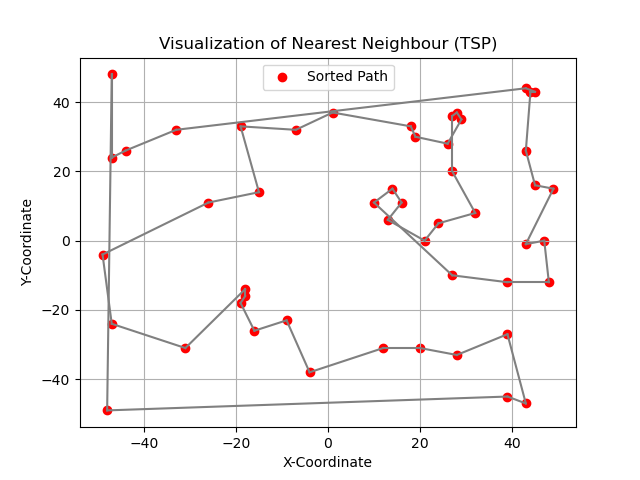
\includegraphics[width=1.1\linewidth]{assets/Img/NearestVisual.png}
            \caption{Nearest Neighbour}
            \label{fig:nearest}
      \end{minipage}%
      \begin{minipage}{.48\textwidth}
            \centering
            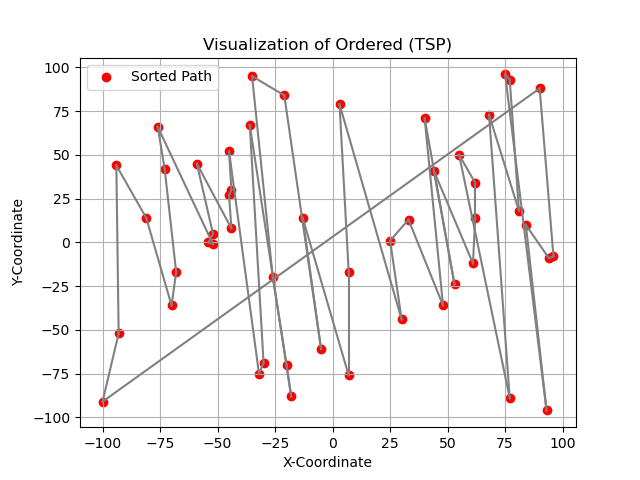
\includegraphics[width=1.1\linewidth]{assets/Img/OrdVisual.png}
            \caption{Ordenación}
            \label{fig:ordered}
      \end{minipage}
\end{figure}
\begin{figure}[H]
      \centering
      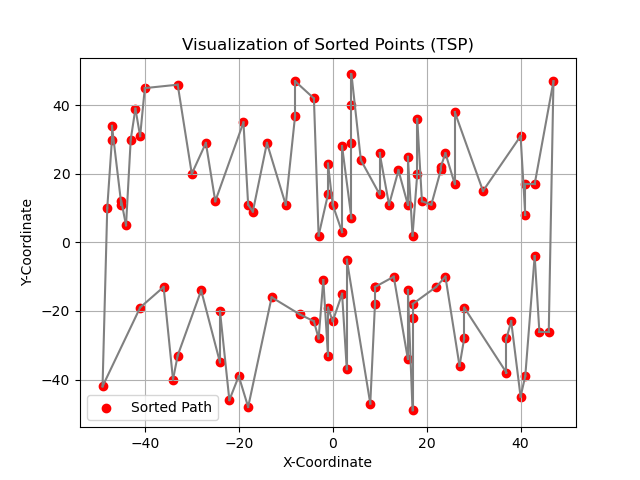
\includegraphics[width=0.6\linewidth]{assets/Img/CircVisual.png}
      \caption{Circular}
      \label{fig:circular}
\end{figure}
Una vez graficadas, podemos ver los problemas principales de cada uno de los algoritmos,
en el caso de \textit{Nearest Neighbour}, se puede apreciar que la distancia de cierre
es muy grande, sin embargo, aparenta un camino parecido al óptimo, en el caso de 
\textit{Ordenación}, se puede apreciar que, mientras los puntos x están cerca, los saltos
en y son muy grandes, y además la distancia de cierre es máxima, en el caso de \textit{Circular},
se puede apreciar que los saltos en y son más pequeños y la distancia de cierre es menor.
\\ \\ 
De este análisis visual, podemos deducir que el algoritmo \textit{Nearest Neighbour} es el
que mejor resultado proporciona, le sigue \textit{Circular} y por último \textit{Ordenación}.
Podríamos dejar el estudio aquí, sin embargo, se proponen maneras de mejorar los algoritmos.
\subsection{Mejoras}
Para mejorar y comparar los algoritmos, comenzamos notando que en el caso de 
\textit{Nearest Neighbour}, la elección del punto de partida nos proporciona un camino
distinto, por lo que, para mejorar la precisión del algoritmo, se puede ejecutar
el algoritmo con distintos puntos de partida y quedarnos con el mejor resultado.
En los casos de \textit{Ordenación} y \textit{Circular}, esto no tendría mucho sentido, 
sin embargo podríamos jugar con la ordenación respecto de un eje u otro, o con la
división en dos partes, respectivamente, para mejorar la precisión de los mismos.
\\ \\
Este tipo de mejoras, son sencillas y no suponen un gran aumento en cuanto al tiempo
de ejecución, sin embargo, tampoco suponen una mejora significativa en cuanto a la
precisión. Su mejor virtud es que nos proporcionan una velocidad de ejecución muy
rápida y una precisión aceptable, por lo que, en la práctica, se recomienda su uso,
sin embargo, habrá aplicaciones en las que se necesite una precisión mayor, en cuyo 
caso se recomienda el uso de algoritmos más complejos como $\lambda$-opt o genéticos.
\subsection{Precisión y Tiempos}
En esta sección se proporcionan los tiempos de ejecución de los algoritmos y se comparan
con la precisión de los mismos, para ello, se han ejecutado los algoritmos sobre un entorno
cuya solución óptima se conoce, de esta forma, se puede comparar la solución obtenida
con la solución óptima, el entorno en cuestión es un conjunto de Paises del mundo
que se han dividido en pueblos y ciudades de interés. A continuación mostramos 
los resultados que hemos obtenido:



\end{document}